\documentclass{article}

\PassOptionsToPackage{numbers,sort&compress}{natbib}
\usepackage[final]{neurips_2026}

\usepackage[utf8]{inputenc}
\usepackage[T1]{fontenc}
\usepackage{hyperref}
\usepackage{url}
\usepackage{booktabs}
\usepackage{amsmath}
\usepackage{amsfonts}
\usepackage{microtype}
\usepackage{xcolor}
\usepackage{graphicx}

\title{Bearing Remaining Useful Life Prediction from Vibration Signals under Operating-Condition Shift}

\author{%
  Team 27\\
  ECE 228 Project\\
  University of California San Diego
}

\begin{document}

\maketitle

\begin{abstract}
Remaining useful life (RUL) prediction is central to condition-based maintenance of rotating machinery. 
In rolling bearings, vibration signals provide rich degradation information, but prediction becomes challenging when the test bearing operates under a different speed/load condition from the training bearings. 
We study feature-based RUL prediction on the XJTU-SY bearing dataset under a trajectory-level cross-condition protocol. 
Horizontal and vertical vibration signals are converted into time-domain, frequency-domain, and wavelet-domain features. 
We compare a classical Ridge regression baseline with LSTM, TCN, Transformer, and Latent ODE sequence models. 
Feature-level ablation shows that compact train-only feature screening reduces redundancy in the expanded feature space, while sequence-length analysis highlights the trade-off between longer temporal context and short-trajectory coverage. 
Under the strict full-coverage setting using wavelet-only features with sequence length $K=40$, LSTM achieves the best average cross-condition MAE of 0.176, outperforming Ridge regression with MAE 0.270. 
The results suggest that vibration-derived wavelet representations and neural sequence models improve cross-condition RUL prediction, although operating-condition shift remains a major source of error.
\end{abstract}

\section{Introduction}

Rolling bearings are widely used in rotating machinery, and their failures can lead to unexpected downtime, safety risks, and high maintenance cost. 
Vibration-based monitoring is a standard approach for bearing diagnostics and prognostics because mechanical defects often induce changes in signal amplitude and frequency content \citep{randall2011rolling}. 
Remaining useful life prediction aims to estimate how long a component can continue operating before failure, enabling condition-based maintenance decisions \citep{jardine2006review}.

Data-driven RUL prediction has benefited from machine learning and neural sequence models, but a key challenge is generalization across operating conditions. 
Bearings running under different speed and load settings may exhibit different degradation trajectories even when the sensor modality is the same. 
Therefore, evaluating only random windows from mixed conditions can overestimate performance. 
In this work, we focus on a stricter setting: models are trained and validated on two operating conditions and tested on a completely unseen condition.

Our main question is whether vibration-derived feature representations, especially wavelet-domain features, can improve RUL prediction under operating-condition shift. 
We make three contributions. 
First, we construct a leakage-free feature-based pipeline using time-domain, frequency-domain, and wavelet-domain vibration features from both acceleration channels. 
Second, we evaluate feature settings and top-$k$ train-only feature screening to study redundancy and compact feature selection. 
Third, we compare Ridge regression and neural sequence models under leave-one-condition-out evaluation using bearing-level metrics.

\section{Related Work}

Bearing prognostics has been studied using both signal-processing features and learning-based models. 
Classical vibration analysis often relies on time-domain statistics, frequency-domain descriptors, and wavelet-based decompositions to characterize amplitude changes, impulsive components, and frequency-band energy distribution \citep{randall2011rolling,daubechies1988orthonormal}. 
Recent RUL prediction methods combine feature extraction with deep neural models to capture degradation dynamics from sensor sequences \citep{wang2018hybrid,dhungana2026remaining}.

Sequence models are commonly used for temporal degradation modeling. 
LSTM networks model long-range dependencies through recurrent gates \citep{hochreiter1997lstm}. 
Temporal convolutional networks provide a convolutional alternative for sequence modeling \citep{bai2018tcn}. 
Transformers use self-attention to capture dependencies across temporal windows \citep{vaswani2017attention}. 
Latent ODE and neural ODE models provide continuous-time sequence modeling tools \citep{chen2018neuralode}. 
Unlike work that primarily evaluates within-condition interpolation, this project emphasizes trajectory-level cross-condition generalization on XJTU-SY.

\section{Method}

We propose a feature-based framework for predicting the remaining useful life of rolling bearings under varying operating conditions. 
As shown in Figure~\ref{fig:pipeline}, the pipeline transforms raw horizontal and vertical vibration measurements into time-domain, frequency-domain, and wavelet-domain features. 
These features are organized into multiple feature settings, including original time-frequency features, wavelet-only features, all-expanded features, and compact top-$k$ subsets selected through train-only feature screening. 
For neural sequence models, each run-to-failure trajectory is converted into fixed-length temporal windows. 
We compare Ridge regression with LSTM, TCN, Transformer, and Latent ODE models, and evaluate them using a leave-one-condition-out cross-condition protocol.

\begin{figure}[t]
    \centering
    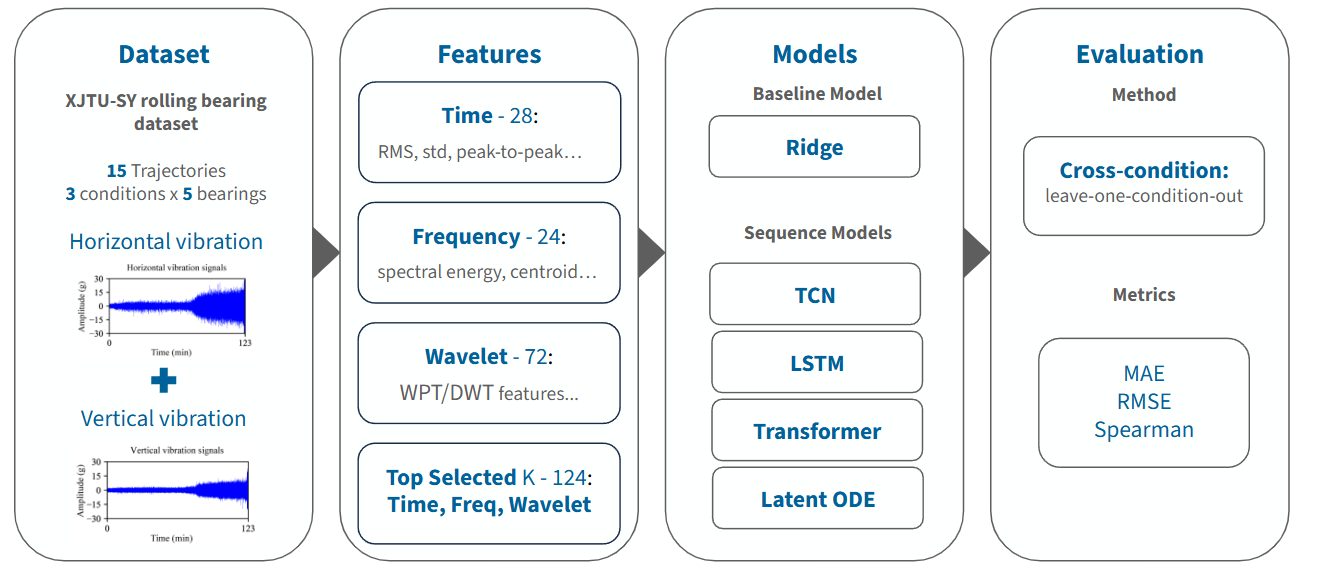
\includegraphics[width=\textwidth]{figures/pipeline.png}
    \caption{Overview of the proposed feature-based RUL prediction pipeline.}
    \label{fig:pipeline}
\end{figure}

\subsection{Dataset}

We use the XJTU-SY rolling bearing accelerated life test dataset \citep{lei2019xjtu} as a standard benchmark. 
The dataset contains 15 run-to-failure trajectories sampled under three operating conditions, with five bearings for each condition. 
As summarized in Table~\ref{tab:xjtu_conditions}, the conditions differ in rotational speed and radial load, resulting in distinct degradation trajectories under different operating regimes.

\begin{table}[t]
\centering
\caption{Operating conditions in the XJTU-SY dataset.}
\label{tab:xjtu_conditions}
\begin{tabular}{cccc}
\toprule
Condition & Speed & Load & Bearing trajectories \\
\midrule
C1 & 35 Hz & 12 kN & 5 trajectories: B1-1 to B1-5 \\
C2 & 37.5 Hz & 11 kN & 5 trajectories: B2-1 to B2-5 \\
C3 & 40 Hz & 10 kN & 5 trajectories: B3-1 to B3-5 \\
\bottomrule
\end{tabular}
\end{table}

Each trajectory contains vibration data recorded until bearing failure. 
Each measurement includes horizontal and vertical acceleration signals sampled at 25.6 kHz, with 32,768 data points collected over 1.28 seconds at one-minute intervals. 
We use only features extracted from the two acceleration channels. 
Failure mode annotations are treated as metadata and are not used as model inputs.

Figure~\ref{fig:example_vibration_signals} shows example horizontal and vertical vibration signals from one run-to-failure trajectory. 
The signal amplitude becomes more pronounced near the end of the trajectory, indicating that the raw vibration measurements contain degradation-related information.

\begin{figure}[t]
    \centering
    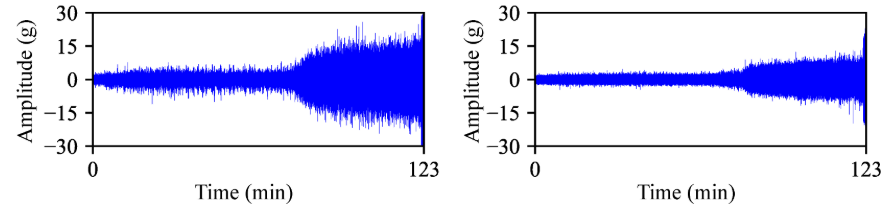
\includegraphics[width=0.82\textwidth]{figures/example_vibration_signals.png}
    \caption{Example horizontal and vertical vibration signals from one XJTU-SY run-to-failure trajectory.}
    \label{fig:example_vibration_signals}
\end{figure}

\subsection{Problem Formulation}

We treat each bearing as a run-to-failure trajectory. 
For trajectory $b$, let $N_b$ denote the number of measurements, and let $\mathbf{x}_{b,t}\in\mathbb{R}^{d}$ be the vibration-derived feature vector at time $t\in\{0,\ldots,N_b-1\}$. 
The normalized remaining useful life target is defined as
\[
y_{b,t}=\frac{N_b-1-t}{N_b-1}.
\]
This is a constructed supervised label and does not imply linear physical degradation.

The prediction task is to learn a mapping from vibration-derived representations to normalized RUL:
\[
\hat{y}_{b,t}=f_{\theta}(\mathbf{x}_{b,t})
\quad \text{or} \quad
\hat{y}_{b,t}=f_{\theta}(\mathbf{X}_{b,t}),
\]
where $\mathbf{X}_{b,t}$ denotes a temporal feature window and $\theta$ denotes model parameters. 
The first formulation is used for Ridge regression, while the second is used for sequence models.

\subsection{Vibration Feature Extraction}

For each vibration measurement, we extract features from the horizontal and vertical acceleration channels and concatenate them into a single feature vector. 
We consider three sets of complementary features: time-domain, frequency-domain, and wavelet-domain features, as summarized in Table~\ref{tab:feature_groups}.

Time-domain features capture the amplitude statistics and impulse characteristics of the vibration signal. 
For each channel, we compute 14 statistics, including root mean square, standard deviation, peak-to-peak value, skewness, kurtosis, energy, peak coefficient, impulse coefficient, and shape coefficient. 
This yields 28 time-domain features across the two channels.

Frequency-domain features describe the spectral distribution of vibration energy. 
For each channel, we compute 12 descriptors, including spectral energy, spectral centroid, spectral entropy, dominant frequency, bandwidth energy, and bandwidth energy ratio. 
This yields 24 frequency-domain features.

Wavelet-domain features describe the distribution of vibration energy across different frequency bands during bearing operation. 
We employ the Daubechies-4 wavelet \citep{daubechies1988orthonormal} and perform a three-level decomposition. 
The level-3 Wavelet Packet Transform decomposes each signal into $2^3=8$ terminal frequency bands, from which energy, root mean square, and energy ratios are extracted. 
We also summarize the discrete wavelet transform coefficient sets $cA_3$, $cD_3$, $cD_2$, and $cD_1$ using mean, variance, and energy. 
This gives
\[
(8 \times 3 + 4 \times 3) \times 2 = 72
\]
wavelet-domain features in total.

\begin{table}[t]
\centering
\caption{Vibration feature groups used in this study.}
\label{tab:feature_groups}
\begin{tabular}{c c p{8.2cm}}
\toprule
Feature group & Dim. & Description \\
\midrule
Time-domain & 28 & Amplitude and impulse statistics from two channels, including RMS, standard deviation, peak-to-peak value, skewness, kurtosis, and energy. \\
Frequency-domain & 24 & Spectral descriptors from two channels, including spectral energy, spectral centroid, spectral entropy, dominant frequency, bandwidth energy, and bandwidth energy ratio. \\
Wavelet-domain & 72 & Daubechies-4 level-3 WPT and DWT statistics, including band energy, RMS, energy ratio, coefficient mean, variance, and energy. \\
\bottomrule
\end{tabular}
\end{table}

\subsection{Feature Settings and Train-only Feature Screening}

After extracting features from the time, frequency, and wavelet domains, we organize them into several feature settings for comparison. 
The original setting includes time-domain and frequency-domain features, totaling 52 features. 
The wavelet-only setting includes only the 72 wavelet-domain features. 
The all-expanded setting concatenates the original features with the wavelet-only features, totaling 124 features. 
We also evaluate compact top-$k$ feature sets selected from the all-expanded feature space, where $k \in \{10,20,30\}$.

The purpose of the top-$k$ setting is to reduce redundancy in the expanded feature space. 
Although the all-expanded setting contains more information, it may also introduce irrelevant features, multicollinearity, and condition-specific noise. 
Motivated by feature selection criteria based on correlation, monotonicity, and robustness \citep{dhungana2026remaining}, we rank each feature using a screening score based solely on training data:
\[
S_j = 0.5 C_j + 0.4 M_j + 0.1 R_j,
\]
where $C_j$ measures the correlation between feature $j$ and the normalized RUL target, $M_j$ measures the monotonic trend of the feature over the bearing lifetime, and $R_j$ measures robustness under local fluctuations. 
Features with the highest $S_j$ values are selected as the top-$k$ feature set.

Feature screening is performed independently for each split using only training trajectories. 
Validation and test trajectories are not used when calculating $C_j$, $M_j$, $R_j$, or selecting the top-$k$ features. 
This prevents information from the evaluation conditions from leaking into the training process.

\begin{table}[t]
\centering
\caption{Feature settings evaluated in this study.}
\label{tab:feature_settings}
\begin{tabular}{c c p{7.8cm}}
\toprule
Feature setting & Dim. & Description \\
\midrule
Original & 52 & Time-domain and frequency-domain features. \\
Wavelet-only & 72 & Wavelet-domain features only. \\
All-expanded & 124 & Concatenation of original and wavelet-only features. \\
Top-$k$ & $k$ & Top-$k$ features selected from the all-expanded feature space using training trajectories only. \\
\bottomrule
\end{tabular}
\end{table}

\subsection{Sequence Construction}

Ridge regression uses the current feature vector $\mathbf{x}_{b,t}$ directly and does not require temporal sequence construction. 
For neural sequence models, we construct fixed-length temporal windows from each bearing trajectory. 
Given sequence length $K$, the input window at time $t$ is
\[
\mathbf{X}_{b,t} =
[\mathbf{x}_{b,t-K+1}, \mathbf{x}_{b,t-K+2}, \ldots, \mathbf{x}_{b,t}],
\]
with prediction target $y_{b,t}$ at the final time step.

Sequences are generated independently within each bearing trajectory. 
No sequence is allowed to cross trajectory boundaries. 
The sequence length $K$ determines how much historical information is available to the model. 
A larger $K$ provides longer degradation history, but it may exclude short trajectories that do not contain enough measurements to form complete windows. 
Therefore, $K$ is selected using validation performance together with a trajectory coverage check.

\subsection{Prediction Models}

We evaluate five prediction models. 
Ridge regression serves as a classical feature-based baseline and maps the current feature vector $\mathbf{x}_{b,t}$ directly to normalized RUL. 
The remaining models are neural sequence models that take temporal windows $\mathbf{X}_{b,t}$ as input.

The LSTM captures temporal dependencies through recurrent hidden states \citep{hochreiter1997lstm}. 
The TCN models local temporal patterns using one-dimensional convolutions over the feature window \citep{bai2018tcn}. 
The Transformer uses self-attention with positional encoding to capture dependencies across the full sequence \citep{vaswani2017attention}. 
Latent ODE is included as a continuous-time sequence modeling baseline, where hidden dynamics are represented by a neural ordinary differential equation \citep{chen2018neuralode}. 
All neural models output a scalar prediction for the final time step of the input window.

\subsection{Training, Validation, and Model Selection}

All preprocessing is performed inside each split. 
Feature scaling parameters are fitted only on training trajectories and are then applied to validation and test trajectories. 
For the top-$k$ settings, feature screening is also performed only on the training trajectories.

For Ridge regression, the regularization strength is selected using validation MAE. 
For neural models, we train with Adam, use early stopping based on validation error, and evaluate the best validation checkpoint on the test condition. 
The test condition is used only once after preprocessing, feature screening, sequence-length selection, and model selection are fixed.

\subsection{Evaluation Protocol}

The main experiment uses a leave-one-condition-out cross-condition protocol. 
In each split, two operating conditions provide training and validation trajectories, while the remaining operating condition is used only for testing. 
Specifically, we evaluate three held-out settings: train on C1/C2 and test on C3, train on C1/C3 and test on C2, and train on C2/C3 and test on C1. 
All splits are performed at the bearing-trajectory level rather than the window level.

We report mean absolute error, root mean squared error, and Spearman correlation. 
MAE measures average absolute prediction error, RMSE penalizes larger errors, and Spearman correlation measures whether the predicted RUL follows the correct ranking trend over the bearing lifetime. 
Metrics are computed for each test bearing first and then averaged across bearings and cross-condition splits.

\section{Results and Analysis}

\subsection{Feature Setting Ablation}

We first evaluate the feature settings using Ridge regression as a diagnostic model. 
Ridge does not use temporal windows, so this experiment isolates the effect of feature representation from sequence modeling. 
As shown in Figure~\ref{fig:feature_ablation_bar}, the compact Top10 setting obtains the lowest average cross-condition MAE among Ridge variants, while the all-expanded setting performs the worst. 
This suggests that directly concatenating all features can introduce redundancy and condition-specific noise.

\begin{figure}[t]
    \centering
    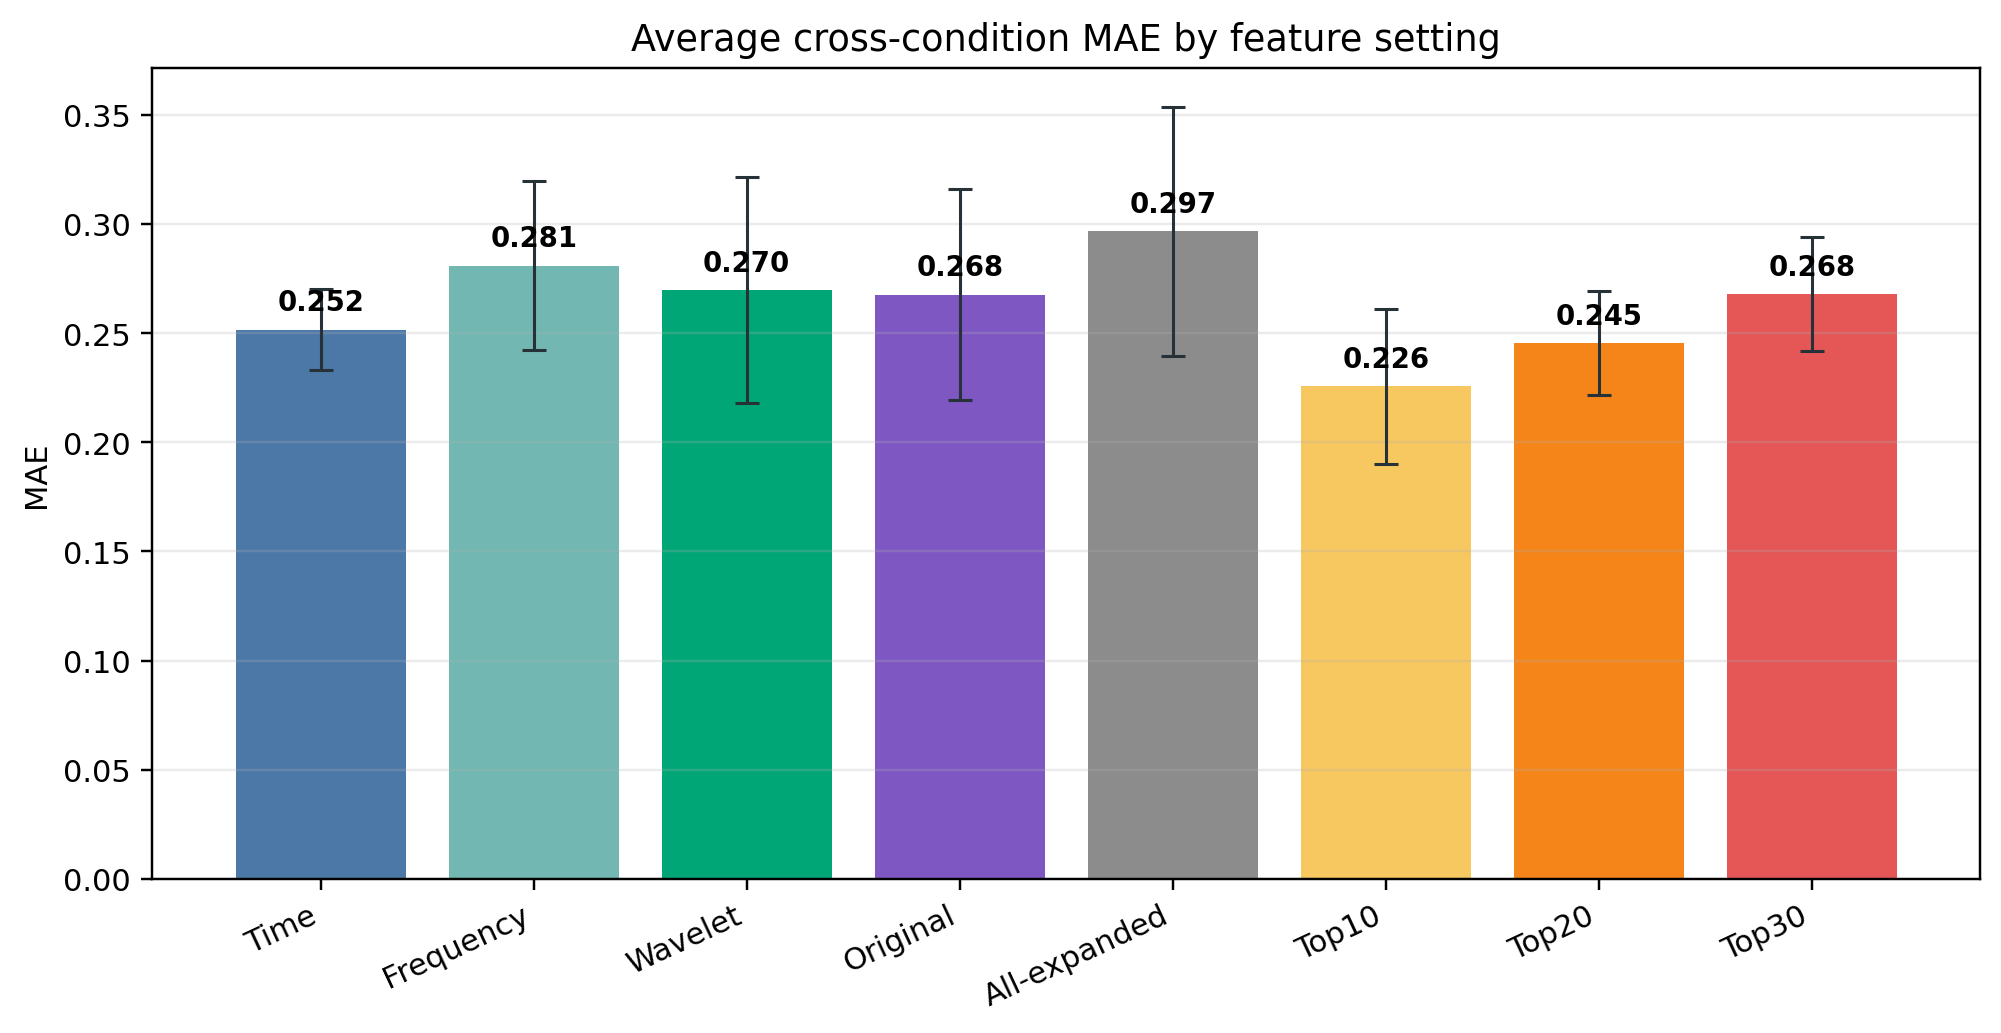
\includegraphics[width=0.88\textwidth]{figures/ridge_feature_ablation_bar.png}
    \caption{Average cross-condition MAE by feature setting using Ridge regression. Error bars show variation across held-out conditions.}
    \label{fig:feature_ablation_bar}
\end{figure}

Figure~\ref{fig:topk_composition} shows the average composition of selected top-$k$ features. 
Wavelet features appear consistently in the compact selected subsets, indicating that wavelet-derived information is useful even when the final selected feature set is small. 
However, wavelet-only is not always the best standalone Ridge setting, so we interpret wavelet features as complementary rather than universally sufficient.

\begin{figure}[t]
    \centering
    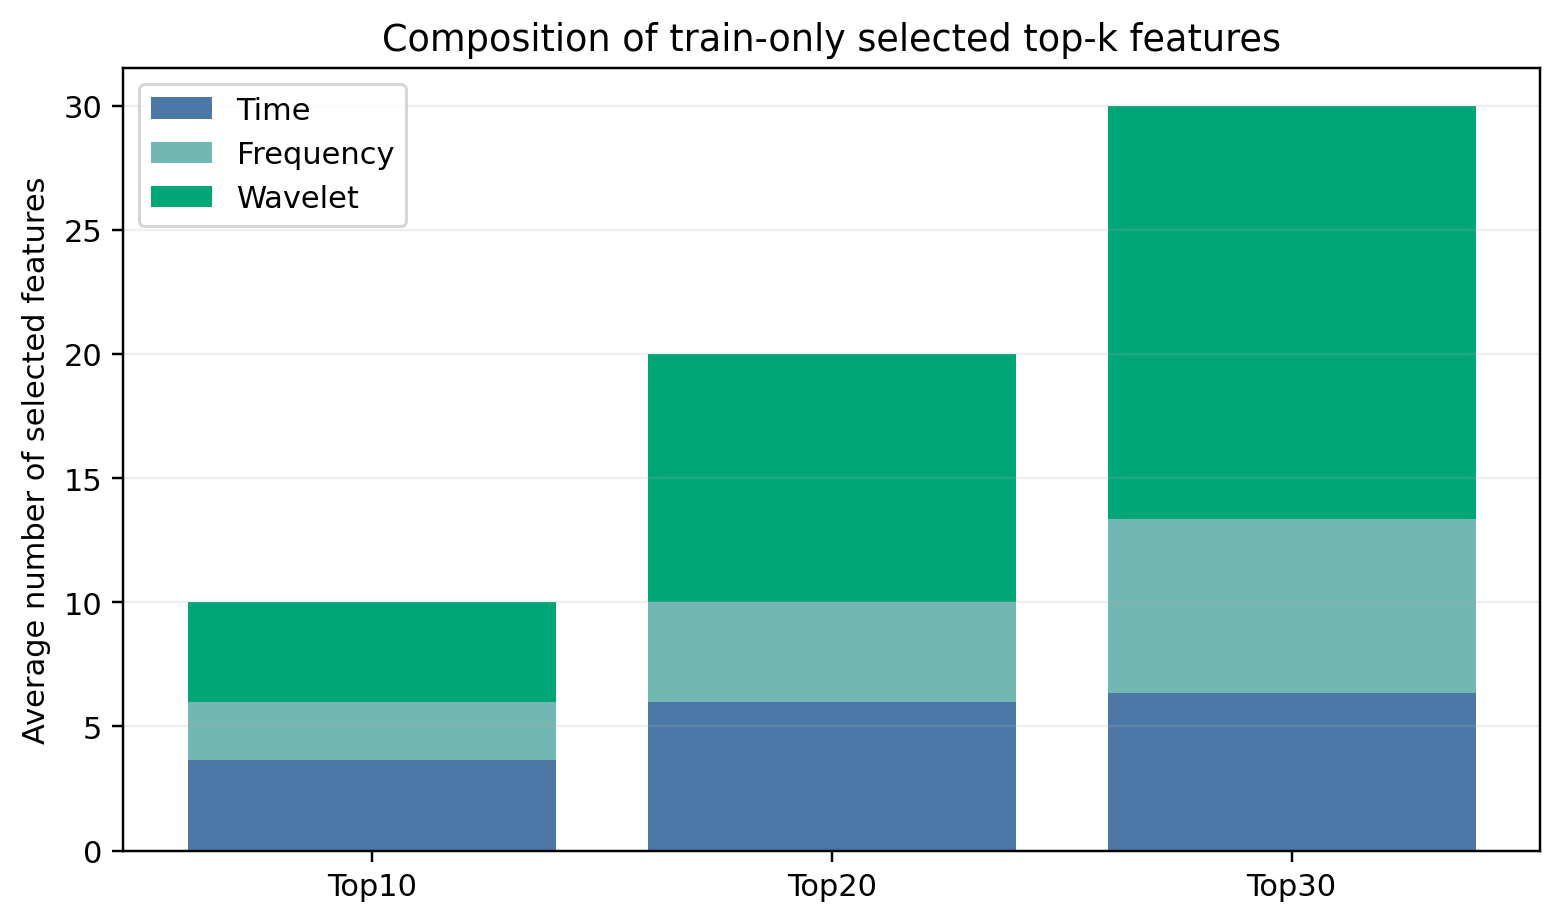
\includegraphics[width=0.72\textwidth]{figures/selected_topk_feature_composition.png}
    \caption{Average composition of train-only selected top-$k$ features across cross-condition splits.}
    \label{fig:topk_composition}
\end{figure}

\subsection{Sequence Length Selection}

We then evaluate sequence length for neural models using wavelet-only features. 
Figure~\ref{fig:k_selection} shows the validation MAE and coverage behavior for different values of $K$. 
Although $K=100$ achieves the lowest raw validation MAE, it does not preserve complete coverage for short trajectories. 
We therefore choose $K=40$ for the main strict experiment because it preserves full train, validation, and test trajectory coverage.

\begin{figure}[t]
    \centering
    
\includegraphics[width=0.95\textwidth]{figures/k_selection_v2_accuracy_coverage.png}
    \caption{Sequence-length selection with validation MAE and trajectory coverage. We use $K=40$ as the strict full-coverage setting.}
    \label{fig:k_selection}
\end{figure}

\subsection{Main Cross-condition Results}

The main cross-condition experiment uses wavelet-only features and $K=40$ for all neural sequence models. 
Table~\ref{tab:main_results} reports the average results over the three held-out conditions. 
LSTM obtains the best average MAE of 0.176 and RMSE of 0.208. 
Transformer obtains a higher MAE but the strongest Spearman correlation among the neural models, indicating better trend consistency. 
All neural sequence models outperform Ridge in MAE, supporting the value of temporal modeling under operating-condition shift.

\begin{table}[t]
\centering
\caption{Main cross-condition results using wavelet-only features and $K=40$.}
\label{tab:main_results}
\begin{tabular}{lccc}
\toprule
Model & MAE & RMSE & Spearman \\
\midrule
LSTM & \textbf{0.176} & \textbf{0.208} & 0.410 \\
Transformer & 0.198 & 0.237 & \textbf{0.493} \\
TCN & 0.224 & 0.267 & 0.427 \\
Latent ODE & 0.233 & 0.268 & 0.297 \\
Ridge & 0.270 & 0.324 & 0.324 \\
\bottomrule
\end{tabular}
\end{table}

\begin{figure}[t]
    \centering
    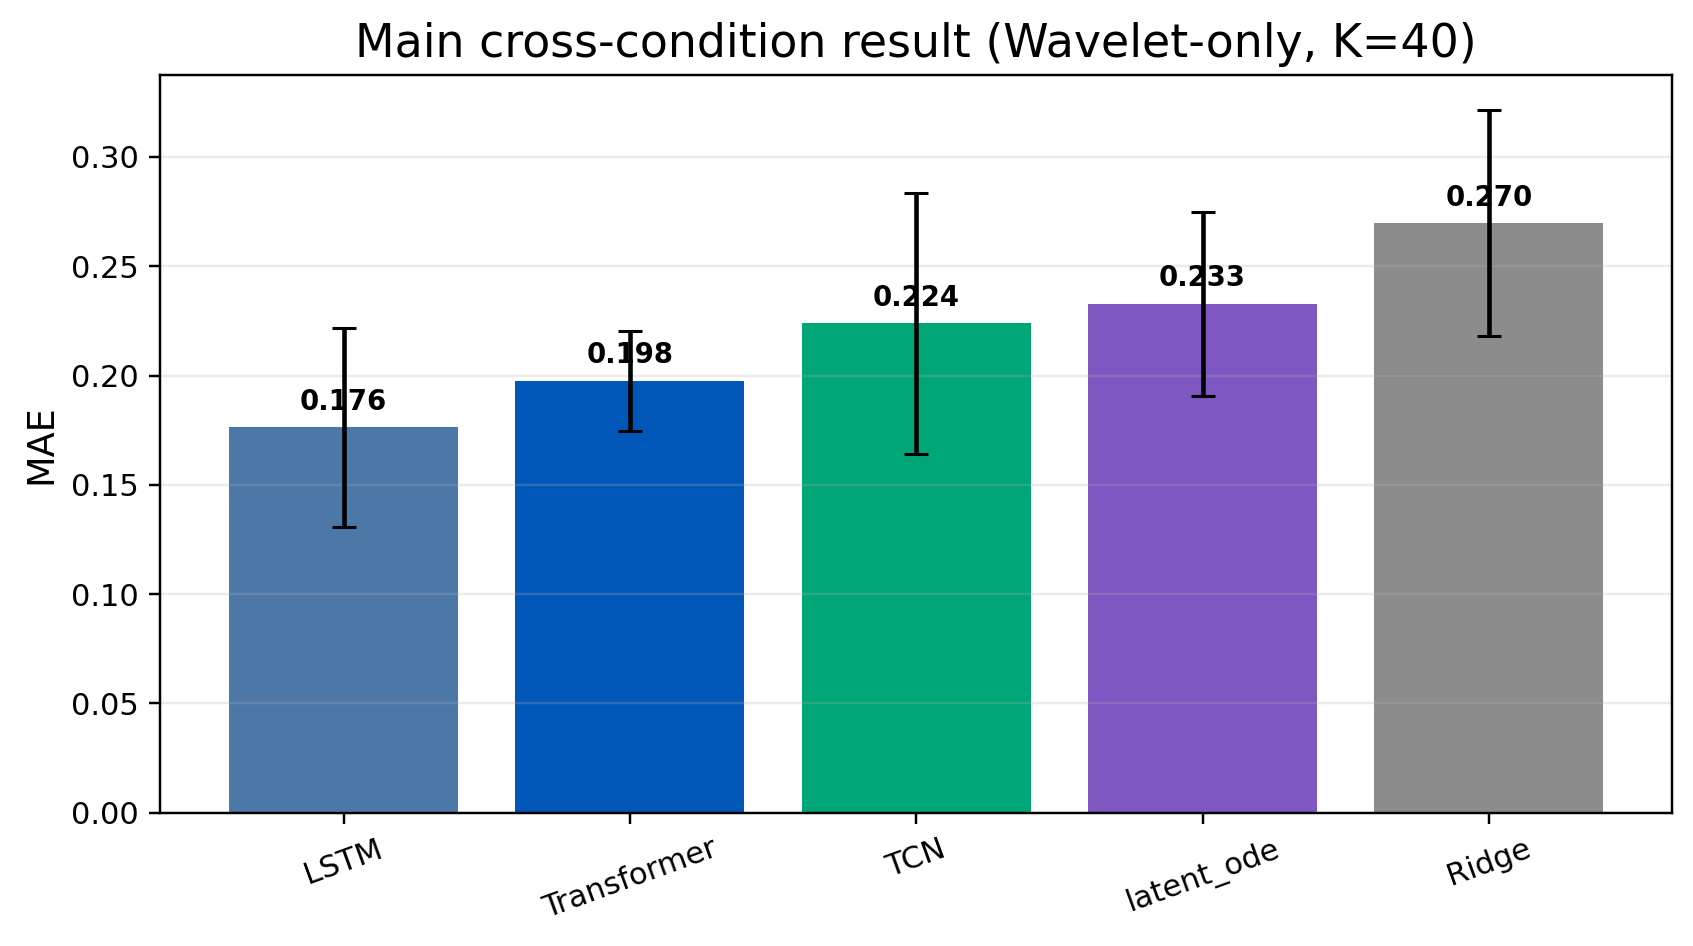
\includegraphics[width=0.82\textwidth]{figures/cross_only_mae_bar_v2.png}
    \caption{Average cross-condition MAE for the main wavelet-only, $K=40$ setting.}
    \label{fig:main_mae}
\end{figure}

Figure~\ref{fig:per_split_heatmap} shows the per-split MAE. 
Performance varies substantially across held-out conditions. 
In particular, C3 is difficult for several models, confirming that operating-condition shift is not a trivial interpolation problem.

\begin{figure}[t]
    \centering
    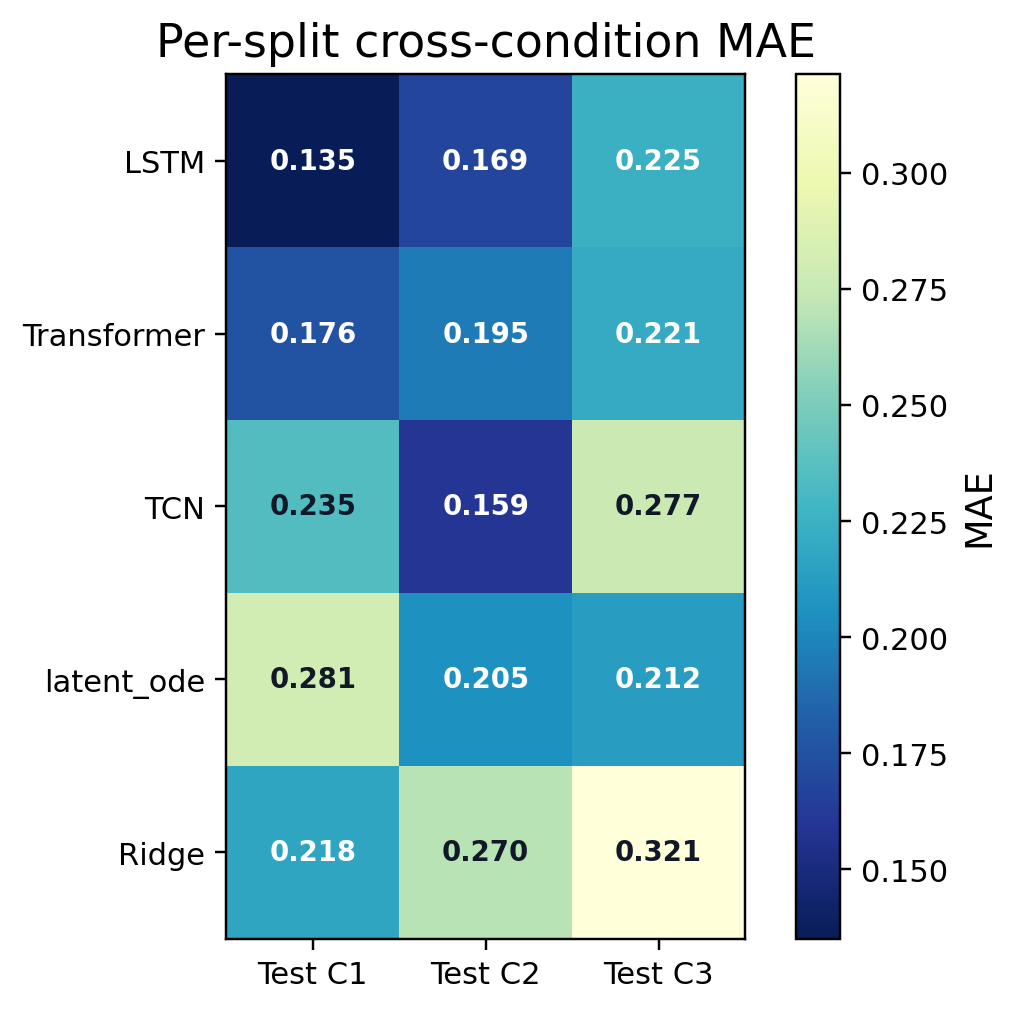
\includegraphics[width=0.62\textwidth]{figures/cross_only_per_split_heatmap_v2.png}
    \caption{Per-split cross-condition MAE. Columns indicate the held-out test condition.}
    \label{fig:per_split_heatmap}
\end{figure}

\section{Discussion}

The experiments show three main findings. 
First, feature representation matters: compact train-only feature screening can improve generalization compared with using all extracted features directly. 
Second, longer sequence windows can improve validation accuracy, but they may exclude short bearing trajectories. 
This motivates using $K=40$ as the strict full-coverage setting rather than selecting the lowest raw validation error alone. 
Third, neural sequence models improve point prediction over Ridge under cross-condition evaluation, but the best model depends on the metric: LSTM has the lowest MAE, while Transformer has stronger rank-trend consistency.

These results should be interpreted conservatively. 
The normalized RUL target is a constructed supervised label rather than a direct physical degradation curve. 
In addition, the XJTU-SY dataset contains only five trajectories per operating condition, so cross-condition evaluation is sensitive to trajectory-level variability. 
Future work could study probabilistic intervals, transfer learning, and physics-informed constraints to improve reliability under stronger distribution shifts.

\section{Conclusion}

We present a leakage-free feature-based framework for bearing RUL prediction under operating-condition shift. 
Using the XJTU-SY dataset, we extract time-domain, frequency-domain, and wavelet-domain features from horizontal and vertical vibration signals, evaluate train-only feature screening, and compare Ridge regression with neural sequence models. 
Under a strict cross-condition protocol, wavelet-only sequence models outperform the Ridge baseline, with LSTM achieving the best MAE. 
The study highlights the importance of trajectory-level evaluation, feature redundancy control, and sequence-length coverage when developing RUL models for engineering deployment.

\bibliographystyle{unsrtnat}
\bibliography{references}

\end{document}
